\documentclass{beamer}
\usepackage{pgfpages}
\setbeameroption{show notes}
\setbeameroption{show notes on second screen=right}

\definecolor{links}{HTML}{2A1B81}
\hypersetup{colorlinks,linkcolor=,urlcolor=links}

\mode<presentation> {

% The Beamer class comes with a number of default slide themes
% which change the colors and layouts of slides. Below this is a list
% of all the themes, uncomment each in turn to see what they look like.

%\usetheme{default}
%\usetheme{AnnArbor}
%\usetheme{Antibes}
%\usetheme{Bergen}
%\usetheme{Berkeley}
%\usetheme{Berlin}
%\usetheme{Boadilla}
\usetheme{CambridgeUS}
%\usetheme{Copenhagen}
%\usetheme{Darmstadt}
%\usetheme{Dresden}
%\usetheme{Frankfurt}
%\usetheme{Goettingen}
%\usetheme{Hannover}
%\usetheme{Ilmenau}
%\usetheme{JuanLesPins}
%\usetheme{Luebeck}
%\usetheme{Madrid}
%\usetheme{Malmoe}
%\usetheme{Marburg}
%\usetheme{Montpellier}
%\usetheme{PaloAlto}
%\usetheme{Pittsburgh}
%\usetheme{Rochester}
%\usetheme{Singapore}
%\usetheme{Szeged}
%\usetheme{Warsaw}

% As well as themes, the Beamer class has a number of color themes
% for any slide theme. Uncomment each of these in turn to see how it
% changes the colors of your current slide theme.

%\usecolortheme{albatross}
%\usecolortheme{beaver}
%\usecolortheme{beetle}
%\usecolortheme{crane}
%\usecolortheme{dolphin}
%\usecolortheme{dove}
%\usecolortheme{fly}
%\usecolortheme{lily}
%\usecolortheme{orchid}
%\usecolortheme{rose}
%\usecolortheme{seagull}
\usecolortheme{seahorse}
%\usecolortheme{whale}
%\usecolortheme{wolverine}

%\setbeamertemplate{footline} % To remove the footer line in all slides uncomment this line
%\setbeamertemplate{footline}[page number] % To replace the footer line in all slides with a simple slide count uncomment this line

%\setbeamertemplate{navigation symbols}{} % To remove the navigation symbols from the bottom of all slides uncomment this line
}
%
%-------------------------------------------------------
% INCLUDE PACKAGES
%-------------------------------------------------------
\usepackage[utf8]{inputenc}
\usepackage[english]{babel}
\usepackage[T1]{fontenc}
\usepackage{helvet}
\usepackage{graphicx} % Allows including images
\usepackage{booktabs} % Allows the use of \toprule, \midrule and \bottomrule in tables
\usepackage{siunitx}
\newcommand{\gc}{\degreeCelsius}
\usepackage{tikz}
\usepackage{listings}
%-------------------------------------------------------
% INCLUDE NOTES
%-------------------------------------------------------
%\setbeameroption{show notes}


%-------------------------------------------------------
% INFORMATION IN THE TITLE PAGE
%-------------------------------------------------------

\title[IntSciProg]{\textbf{Tutorial of GNU/Linux in the console. Module V}}

\subtitle{\textbf{Introduction to Scientific Programming}}


\newcommand\RBox[1]{%
  \tikz\node[draw,rounded corners,align=center,] {#1};%
}  
\author[Curro Pérez-Bernal]
{%
  \texorpdfstring{
    % \begin{columns}
    %   \column{.45\linewidth}
      \centering
      \RBox{Curro Pérez-Bernal\\
        \href{mailto:curropb@uhu.es}{curropb@uhu.es}}
    % \end{columns}
    \vspace{0.5cm}
    \begin{columns}
      \column{.75\linewidth}
      \centering
      \RBox{Integrated Sciences Department --
        University of Huelva}
    \end{columns}
  }
  {John Doe \& Jane Doe}
}
% \author[Jos\'e E. Garc\'{\i}a Ramos]{Jos\'e E. Garc\'{\i}a Ramos}% Your name
% \institute[DCI-UHU]
  
%   \medskip
%   \textit{curropb@uhu.es} % Your email address
  
% \author[Curro P\'erez-Bernal ]{Curro P\'erez Bernal}% Your name
% \institute[DCI-UHU]
  
%   \medskip
%   \textit{curropb@uhu.es} % Your email address

% there must be an empty line above this line - otherwise some unwanted space is added between the university and the country (I do not know why;( )

\date{\today} % Date, can be changed to a custom date

\titlegraphic{\begin{center}\vspace{-0.5cm}\hspace{0.5cm}
\includegraphics[width=0.75\linewidth]{Figs/uhu_ceafmc_fisum_isp.png}\end{center}}


%-------------------------------------------------------
% THE BODY OF THE PRESENTATION
%-------------------------------------------------------

\begin{document}

%-------------------------------------------------------
% THE TITLEPAGE
%-------------------------------------------------------

%{\1% % this is the name of the PDF file for the background
\begin{frame}[plain,noframenumbering] % the plain option removes the header from the title page, noframenumbering removes the numbering of this frame only
  \titlepage % call the title page information from above
\end{frame}%}


\begin{frame}{Chapter Outline}{}
\tableofcontents
\end{frame}

\section{User Management}
%%%%%%%%%%%%%%%%%%%%%%%%%%%%%%%%%%%%%%%%%%%%%%%%%%%%%%%%%%%%%%%%%%%%%%%%%%%% 
%%%%%%%%%%%%%%%%%%%%%%%%%%%%%%%%%%%%%%%%%%%%%%%%%%%%%%%%%%%%%%%%%%%%%%%%%%%% 
%%%%%%%%%%%%%%%%%%%%%%%%%%%%%%%%%%%%%%%%%%%%%%%%%%%%%%%%%%%%%%%%%%%%%%%%%%%% 
%%%%%%%%%%%%%%%%%%%%%%%%%%%%%%%%%%%%%%%%%%%%%%%%%%%%%%%%%%%%%%%%%%%%%%%%%%%% 
\begin{frame}[t,fragile]{Adding an user to the system}
  % ------------------------------------------------------

\vspace{-0.4cm}
  \begin{block}{Adding users with the \alert{\texttt{adduser}} command}
    {\footnotesize
Easy way to add users to the system with a console interactive application. \\Syntax is \alert{\texttt{adduser} \emph{username}} and the new user's password is defined on the fly.}

{\scriptsize
  \begin{lstlisting}
$ sudo adduser bobby
[sudo] password for alice: 
...
Enter new UNIX password: 
Retype new UNIX password: 
passwd: password updated successfully
Changing the user information for bobby
Enter the new value, or press ENTER for the default
	Full Name []: Bobby Doe
........
Is the information correct? [Y/n] y
  \end{lstlisting}
}
    {\footnotesize
If the new user is expected to have administration privileges (e.g.\ use of \texttt{sudo})  it has to be added to the \texttt{admin} group. This can be done with the commands \\ \alert{\texttt{usermod -aG sudo}} \emph{username} or \alert{\texttt{adduser } \emph{username} \texttt{sudo}}.}

  \end{block}
  
%%%%%%%%%%%%%%%%%%%%%%%%%%%%%%%%%%%%%%%%%%%%%%%%%%%%%%%%%%%%%%%%%%%%%%%%%%%%%%%%%%
\note{
{\tiny

Notes Module V
}
}
\end{frame}
%%%%%%%%%%%%%%%%%%%%%%%%%%%%%%%%%%%%%%%%%%%%%%%%%%%%%%%%%%%%%%%%%%%%%%%%%%%% 
%%%%%%%%%%%%%%%%%%%%%%%%%%%%%%%%%%%%%%%%%%%%%%%%%%%%%%%%%%%%%%%%%%%%%%%%%%%% 
\begin{frame}[t,fragile]{Removing an user from the system}
  % ------------------------------------------------------


  \begin{block}{Removing users with the \alert{\texttt{deluser}} command}
    {\footnotesize
A user removal is accomplished with the command: \alert{\texttt{deluser} \emph{username}}\\ 
If the user home directory has to be deleted too then the option \texttt{{-}-remove-home} needs to be included. The similar command \alert{\texttt{delgroup}} is used to remove unwanted user groups.}

{\footnotesize
  \begin{lstlisting}
$ sudo deluser --remove-home bobby
[sudo] password for alice: 
Looking for files to backup/remove ...
Removing files ...
Removing user `bobby' ...
Warning: group `bobby' has no more members.
Done.
$ sudo delgroup bobby
The group `bobby' does not exist.
$ cat /etc/group | grep bobby
$ 
  \end{lstlisting}
}

  \end{block}
  
%%%%%%%%%%%%%%%%%%%%%%%%%%%%%%%%%%%%%%%%%%%%%%%%%%%%%%%%%%%%%%%%%%%%%%%%%%%%%%%%%%
\note{
{\tiny

Notes Module V
}
}
\end{frame}
%%%%%%%%%%%%%%%%%%%%%%%%%%%%%%%%%%%%%%%%%%%%%%%%%%%%%%%%%%%%%%%%%%%%%%%%%%%% 
%%%%%%%%%%%%%%%%%%%%%%%%%%%%%%%%%%%%%%%%%%%%%%%%%%%%%%%%%%%%%%%%%%%%%%%%%%%% 
%%%%%%%%%%%%%%%%%%%%%%%%%%%%%%%%%%%%%%%%%%%%%%%%%%%%%%%%%%%%%%%%%%%%%%%%%%%% 
%%%%%%%%%%%%%%%%%%%%%%%%%%%%%%%%%%%%%%%%%%%%%%%%%%%%%%%%%%%%%%%%%%%%%%%%%%%% 
\section{Basics of Private/Public Key Approach}
%%%%%%%%%%%%%%%%%%%%%%%%%%%%%%%%%%%%%%%%%%%%%%%%%%%%%%%%%%%%%%%%%%%%%%%%%%%% 
%%%%%%%%%%%%%%%%%%%%%%%%%%%%%%%%%%%%%%%%%%%%%%%%%%%%%%%%%%%%%%%%%%%%%%%%%%%% 
%%%%%%%%%%%%%%%%%%%%%%%%%%%%%%%%%%%%%%%%%%%%%%%%%%%%%%%%%%%%%%%%%%%%%%%%%%%% 
%%%%%%%%%%%%%%%%%%%%%%%%%%%%%%%%%%%%%%%%%%%%%%%%%%%%%%%%%%%%%%%%%%%%%%%%%%%% 
%%%%%%%%%%%%%%%%%%%%%%%%%%%%%%%%%%%%%%%%%%%%%%%%%%%%%%%%%%%%%%%%%%%%%%%%%%%% 
%%%%%%%%%%%%%%%%%%%%%%%%%%%%%%%%%%%%%%%%%%%%%%%%%%%%%%%%%%%%%%%%%%%%%%%%%%%%
\begin{frame}[t,fragile]{What is the private/public key approach?}
  % ------------------------------------------------------
  \begin{block}{Asymmetric Criptography}
    {\footnotesize
\alert{Asymmetric cryptography} (AC) solves what has always been one of the biggest problems in cryptography: \emph{How can you send someone a coded message without having an opportunity to previously share the code with them?}. AC is based on a pair of associated cryptographic
keys: a \alert{private} key and a \alert{public} key. 

\vspace{0.25cm}
A \textbf{public} key is part of the owner's digital certificate and \emph{it is available for anyone to use}. A \textbf{private} key, however, is protected by and \emph{available only to the owner of the key}. This limited access ensures that communications are kept secure.

\vspace{0.25cm}
The owner of a certificate can use the keys to take advantage of the
security features provided by AC. For example,
he can use a certificate's private key to ``sign''
and encrypt data sent between users and servers, such as messages,
documents, and code objects. The recipient of the signed object can
use the public key contained in the signer's certificate to
decrypt the signature. Such digital signatures ensure the reliability
of an object's origin providing a way of checking the object integrity.
}
  \end{block}
  
%%%%%%%%%%%%%%%%%%%%%%%%%%%%%%%%%%%%%%%%%%%%%%%%%%%%%%%%%%%%%%%%%%%%%%%%%%%%%%%%%%
\note{
{\tiny
Symmetric-key algorithms have their own applications, such as encrypting data for personal use, or for when there are secure channels that the private keys can be shared over.


Notes Module V
}
}
\end{frame}
%%%%%%%%%%%%%%%%%%%%%%%%%%%%%%%%%%%%%%%%%%%%%%%%%%%%%%%%%%%%%%%%%%%%%%%%%%%% 
%%%%%%%%%%%%%%%%%%%%%%%%%%%%%%%%%%%%%%%%%%%%%%%%%%%%%%%%%%%%%%%%%%%%%%%%%%%%
\begin{frame}[t,fragile]{Main Characters and Storyline}
  % ------------------------------------------------------
  \begin{block}{The development of the RSA asymmetryc cryptography}
    {\footnotesize
  \begin{columns}
      \column{.75\textwidth}
      \begin{itemize}
      \item First developments in 1969 at the UK intelligence agency. 
      \item James H. Ellis Ellis and Clifford Cock (RSA), and  Malcolm J. Williamson (D-H key exchange)
      \item \alert{Classified} work. Publicly acknowledged in 1997.
      \item Whitfield Diffie and Martin Hellman designed the \alert{Diffie-Hellman key exchange} in 1976.
      \item  Ron Rivest, Adi Shamir and Leonard Adleman in MIT found a \alert{one-way function} that is the base of the RSA algorithm in 1977.
      \item The idea was patented in 1983 by MIT, but only at the early days of the internet the RSA algorithm began to see widespread adoption.
      \end{itemize}
      \column{.25\textwidth}
      \begin{center}
        % \onslide*{2}{
        % \includegraphics[angle=0,width=5cm]{./Figs/Diagram1.eps}}
        % \onslide*{3}{
        
\includegraphics[angle=0,width=0.95\linewidth]{./Figs/content.jpeg}%}
      \end{center}
    \end{columns}
      
    }
  \end{block}
  
%%%%%%%%%%%%%%%%%%%%%%%%%%%%%%%%%%%%%%%%%%%%%%%%%%%%%%%%%%%%%%%%%%%%%%%%%%%%%%%%%%
\note{
{\tiny

Notes Module V
}
}
\end{frame}
%%%%%%%%%%%%%%%%%%%%%%%%%%%%%%%%%%%%%%%%%%%%%%%%%%%%%%%%%%%%%%%%%%%%%%%%%%%% 
%%%%%%%%%%%%%%%%%%%%%%%%%%%%%%%%%%%%%%%%%%%%%%%%%%%%%%%%%%%%%%%%%%%%%%%%%%%% 
\begin{frame}[t,fragile]{Example of the RSA algorithm}
  % ------------------------------------------------------
  \begin{block}{ RSA basis: difficult factorization of large integers}
    {\footnotesize
      The public key consists of two numbers where one is the product of \alert{two large prime numbers} (trapdoor function). The private key is derived from the same prime numbers. The larger the numbers the safer the key. Let's encrypt the number \texttt{4}.
  \begin{columns}
      \column{.6\textwidth}
      \begin{itemize}
      \item Select two primes, e.g.~ $P = 23$ and $Q = 67$ and $n=PQ$.
        \item Carmichael's Totient function $L(n) = lcm(p-1,q-1)$
        \item Modular inverse $d*e = 1~ mod~ L(n)$
        \item Public key: $\{n, e\}$.
        \item Private Key: $\{n, d\}$.
        \item Ciphertext $c = m^e mod n$
        \item Decrypt $m = c^d mod n$
        \end{itemize}
      \column{.4\textwidth}
{\scriptsize
  \begin{lstlisting}
    m = 4
    n = 1541.
    L(1541) = 748
    e = 53, d = 137
    Public key (1541, 53)
    Private key (1541, 137)
    c = 542
    m = 4
  \end{lstlisting}
}
    \end{columns}
      
    }
  \end{block}
  
%%%%%%%%%%%%%%%%%%%%%%%%%%%%%%%%%%%%%%%%%%%%%%%%%%%%%%%%%%%%%%%%%%%%%%%%%%%%%%%%%%
\note{
{\tiny

Notes Module V
}
}
\end{frame}
%%%%%%%%%%%%%%%%%%%%%%%%%%%%%%%%%%%%%%%%%%%%%%%%%%%%%%%%%%%%%%%%%%%%%%%%%%%% 
%%%%%%%%%%%%%%%%%%%%%%%%%%%%%%%%%%%%%%%%%%%%%%%%%%%%%%%%%%%%%%%%%%%%%%%%%%%% 
%%%%%%%%%%%%%%%%%%%%%%%%%%%%%%%%%%%%%%%%%%%%%%%%%%%%%%%%%%%%%%%%%%%%%%%%%%%% 
%%%%%%%%%%%%%%%%%%%%%%%%%%%%%%%%%%%%%%%%%%%%%%%%%%%%%%%%%%%%%%%%%%%%%%%%%%%% 
\section{Securely Login in Remote Systems}
%%%%%%%%%%%%%%%%%%%%%%%%%%%%%%%%%%%%%%%%%%%%%%%%%%%%%%%%%%%%%%%%%%%%%%%%%%%% 
%%%%%%%%%%%%%%%%%%%%%%%%%%%%%%%%%%%%%%%%%%%%%%%%%%%%%%%%%%%%%%%%%%%%%%%%%%%% 
%%%%%%%%%%%%%%%%%%%%%%%%%%%%%%%%%%%%%%%%%%%%%%%%%%%%%%%%%%%%%%%%%%%%%%%%%%%% 
%%%%%%%%%%%%%%%%%%%%%%%%%%%%%%%%%%%%%%%%%%%%%%%%%%%%%%%%%%%%%%%%%%%%%%%%%%%% 
%%%%%%%%%%%%%%%%%%%%%%%%%%%%%%%%%%%%%%%%%%%%%%%%%%%%%%%%%%%%%%%%%%%%%%%%%%%% 
%%%%%%%%%%%%%%%%%%%%%%%%%%%%%%%%%%%%%%%%%%%%%%%%%%%%%%%%%%%%%%%%%%%%%%%%%%%%
\begin{frame}[t,fragile]{Secure login in remote systems}
  % ------------------------------------------------------
  \begin{block}{Fundamentals of the \alert{\texttt{ssh}} command}
    {\footnotesize
      The command \alert{\texttt{ssh}} is a powerful tool that allows to login in  remote systema and use \texttt{bash} as we do in the local system.  Let's imagine that we are username \texttt{\alert{bob}} in a local system with hostname \texttt{\alert{HAL}} and we want to log into a remote system \texttt{\alert{EARTH}} with username \texttt{\alert{bobby}}. 
    }
    \vspace{0.2cm}
    \begin{columns}
    
      \column{.6\textwidth}
      {\scriptsize
        \begin{itemize}
          \item The server \texttt{\alert{EARTH}} provides its \alert{public} host(s) key(s) and client checks whether this was the intended host and keeps a cache copy.
        
        \item The client \texttt{\alert{HAL}} then generates a \alert{random key}, encrypted with  the public key(s) sent from the server, and sends back this encrypted key. The server unencrypts the key with its own private host key.

        \item Now both sides have a \alert{common key} unknown to anyone else, which will be used to encrypt the rest of the traffic in the session.
        \end{itemize}
       \phantom{ ..}
      }
      \column{.4\textwidth}
      \begin{center}
      % \onslide*{2}{
      % \includegraphics[angle=0,width=5cm]{./Figs/Diagram1.eps}}
      % \onslide*{3}{
        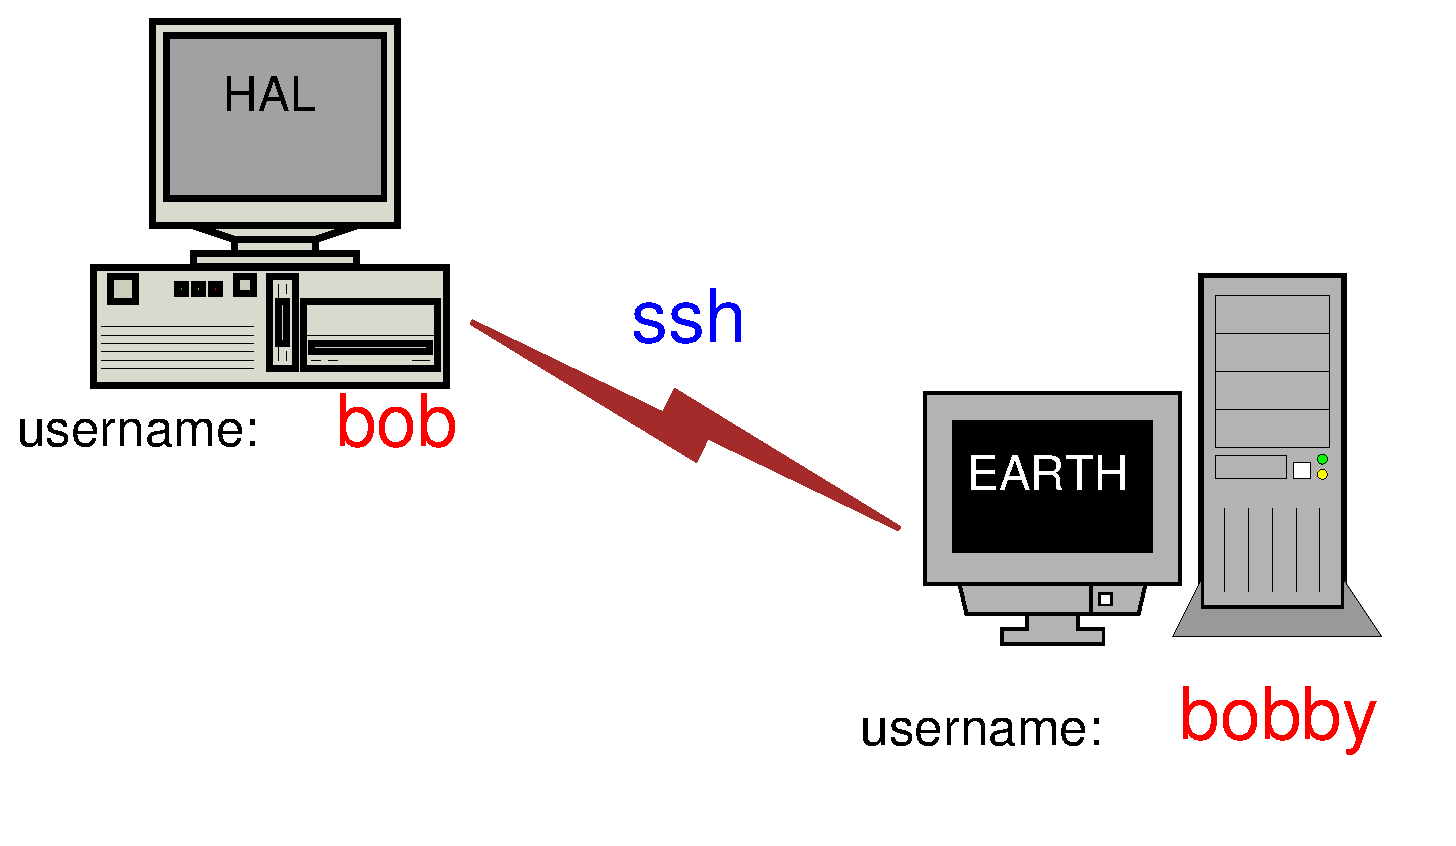
\includegraphics[angle=0,width=\linewidth]{./Figs/Diagram2.eps}%}
      \end{center}
    \end{columns}
  \end{block}
  
  %%%%%%%%%%%%%%%%%%%%%%%%%%%%%%%%%%%%%%%%%%%%%%%%%%%%%%%%%%%%%%%%%%%%%%%%%%%%%%%%%% 
  \note{
    {\tiny
      
      Notes Module V
    }
  }
\end{frame}
%%%%%%%%%%%%%%%%%%%%%%%%%%%%%%%%%%%%%%%%%%%%%%%%%%%%%%%%%%%%%%%%%%%%%%%%%%%% 
%%%%%%%%%%%%%%%%%%%%%%%%%%%%%%%%%%%%%%%%%%%%%%%%%%%%%%%%%%%%%%%%%%%%%%%%%%%% 
\begin{frame}[t,fragile]{Using \alert{\texttt{ssh}}}
  % ------------------------------------------------------


  \begin{block}{Basic command syntax: \alert{\texttt{ssh} \emph{username}@\emph{hostname}}}
    {\footnotesize The first time that a computer is accessed by \texttt{ssh} its public key has to be acknowledged (more details later).}
{\scriptsize
  \begin{lstlisting}
bob@hal:~$ ssh bobby@earth
The authenticity of host 'earth (192.168.1.50)' can't be established.
RSA key fingerprint is 2d:f4:d4:4d:2b:b5:ad:23:0c:f2:db:16:1c:07:27:c1.
Are you sure you want to continue connecting (yes/no)? yes 
Warning: Permanently added 'earth' (RSA) to the list of known hosts.
bobby@earth's password: 
Welcome to Ubuntu 12.04.1 LTS (GNU/Linux 3.2.0-33-generic i686)
Last login: Sun Nov 18 11:18:24 2012 from nostromo
bobby@earth:~$ 
  \end{lstlisting}
}

{\footnotesize\textbf{(a)} In order to be able to login into a computer the package \texttt{openssh-server} has to be installed.\\
\textbf{(b)} The syntax to export the X windows is: 
\texttt{\alert{ssh -X} \emph{\alert{username@computer}}}\\
\textbf{(c)} To close the session use  \texttt{\alert{exit}} or \texttt{CTRL-D}.
}
  \end{block}
  
%%%%%%%%%%%%%%%%%%%%%%%%%%%%%%%%%%%%%%%%%%%%%%%%%%%%%%%%%%%%%%%%%%%%%%%%%%%%%%%%%%
\note{
{\tiny

Notes Module V
}
}
\end{frame}
%%%%%%%%%%%%%%%%%%%%%%%%%%%%%%%%%%%%%%%%%%%%%%%%%%%%%%%%%%%%%%%%%%%%%%%%%%%% 
%%%%%%%%%%%%%%%%%%%%%%%%%%%%%%%%%%%%%%%%%%%%%%%%%%%%%%%%%%%%%%%%%%%%%%%%%%%% 
\begin{frame}[t,fragile]{Running commands in remote systems}
  % ------------------------------------------------------
  \begin{block}{Remote command execution with \alert{\texttt{ssh}}}
    {\footnotesize
The command \alert{\texttt{ssh}} also allows to execute a command in a remote system, passing data streams to and receiving data streams from this command. 

As in the previous example, we are currently working as username \texttt{bob} in a local system with hostname \texttt{HAL}. Now we want to run \texttt{df -h} in a different system whose hostname is \texttt{EARTH} and where our hostname is \texttt{bobby}, appending the output to a file called \texttt{system\_df\_output.dat}. 

      \begin{center}
        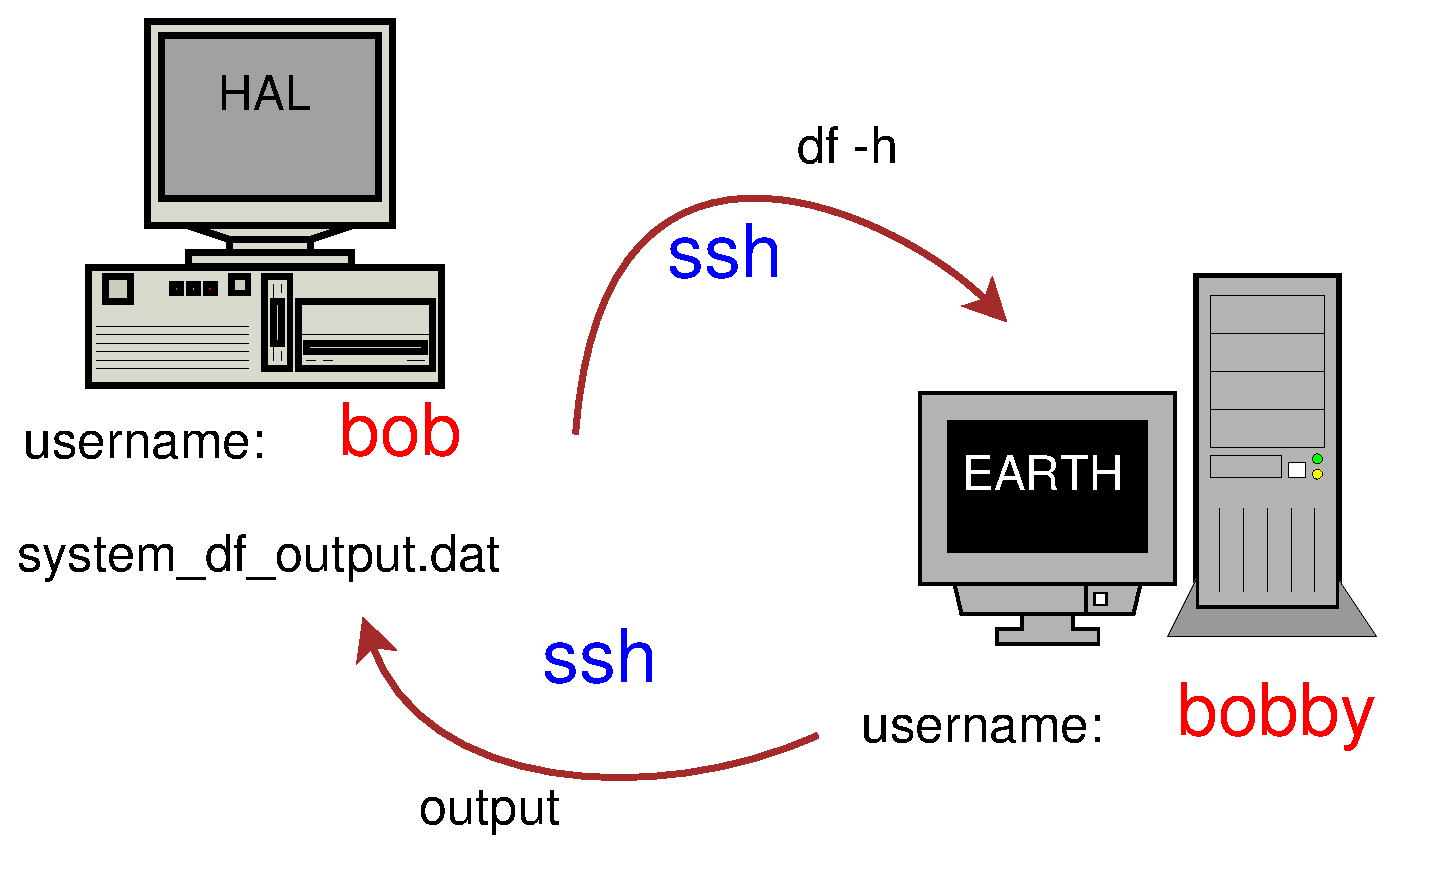
\includegraphics[angle=0,width=5cm]{./Figs/Diagram6.eps}%}
      \end{center}
    }
  \end{block}
  
%%%%%%%%%%%%%%%%%%%%%%%%%%%%%%%%%%%%%%%%%%%%%%%%%%%%%%%%%%%%%%%%%%%%%%%%%%%%%%%%%%
\note{
{\tiny

Notes Module V
}
}
\end{frame}
%%%%%%%%%%%%%%%%%%%%%%%%%%%%%%%%%%%%%%%%%%%%%%%%%%%%%%%%%%%%%%%%%%%%%%%%%%%% 
%%%%%%%%%%%%%%%%%%%%%%%%%%%%%%%%%%%%%%%%%%%%%%%%%%%%%%%%%%%%%%%%%%%%%%%%%%%% 
\begin{frame}[t,fragile]{Remote commands with \alert{\texttt{ssh}}}
  % ------------------------------------------------------


  \begin{block}{Basic command syntax: \alert{\texttt{ssh} \emph{username}@\emph{hostname} \emph{command}}}
    {\footnotesize 
  \begin{lstlisting}
bob@hal:~$ ssh bobby@earth "df -h" >> system_df_output.dat
bob@hal:~$ tail system_df_output.dat
Filesystem            Size  Used Avail Use% Mounted on
/dev/sda2              35G   29G  4.3G  88% /
tmpfs                 628M   12K  628M   1% /lib/init/rw
udev                  623M  272K  623M   1% /dev
tmpfs                 628M  816K  627M   1% /dev/shm
/dev/sdc2             202G   15G  177G   8% /media/usb_disk
/dev/sdc1             391G   21G  370G   6% /media/MSDOS
/dev/sr1              354M  354M     0 100% /media/WD SmartWare
  \end{lstlisting}
}

{\footnotesize The standard input can also be sent to \texttt{\alert{ssh}}}
    {\scriptsize 
  \begin{lstlisting}
bob@hal:~$ echo "Seems magic..." | ssh bobby@earth "cat > magic.dat"
Password:
bob@hal:~$ 
  \end{lstlisting}
}

  \end{block}
  
%%%%%%%%%%%%%%%%%%%%%%%%%%%%%%%%%%%%%%%%%%%%%%%%%%%%%%%%%%%%%%%%%%%%%%%%%%%%%%%%%%
\note{
{\tiny

Notes Module V
}
}
\end{frame}
%%%%%%%%%%%%%%%%%%%%%%%%%%%%%%%%%%%%%%%%%%%%%%%%%%%%%%%%%%%%%%%%%%%%%%%%%%%% 
%%%%%%%%%%%%%%%%%%%%%%%%%%%%%%%%%%%%%%%%%%%%%%%%%%%%%%%%%%%%%%%%%%%%%%%%%%%%
\begin{frame}[t,fragile]{Using silent authentication with \alert{\texttt{ssh}} \textbf{(A)}}
  % ------------------------------------------------------
  \vspace{-0.2cm}
  \begin{block}{\textbf{(A)} Generate user's keypair}
    {\footnotesize The creation by a user of a public/private key pair and its exchange
with a remote system allows the user to login silently withouth
password typing for identification. If user \texttt{bob} in \texttt{hal} wants to login silently in \texttt{earth} the steps are the following:}

{\scriptsize
  \begin{lstlisting}
bob@hal:~$ ssh-keygen -t rsa
Generating public/private rsa key pair.
Enter file in which to save the key (/home/bob/.ssh/id_rsa): [ENTER]
Enter passphrase (empty for no passphrase): [ENTER]
Enter same passphrase again: [ENTER] ...
6e:8a:0d:f7:cb:40:7a:3a:0c:31:18:37:35:37:47:f6 bob@hal.local
The key's randomart image is:
+--[ RSA 2048]----+
|   .o o.+        |
|. o  o + .       |
| + .      E      |
|. o              |
|    o.o +.       |
+-----------------+
bob@hal:~$ 
  \end{lstlisting}
}

% {\footnotesize\textbf{(a)}  We have assumed that the remote directory \texttt{thdir} exists. In case it does not exist use the \alert{\texttt{-r}} option. This option also allows the recursive copy of folders and its contents.\\
% \textbf{(b)} Wildcards and globbing works in the same way as with the usual \texttt{cp} command.
% }

  \end{block}
  
%%%%%%%%%%%%%%%%%%%%%%%%%%%%%%%%%%%%%%%%%%%%%%%%%%%%%%%%%%%%%%%%%%%%%%%%%%%%%%%%%%
\note{
{\tiny

Notes Module V
}
}
\end{frame}
%%%%%%%%%%%%%%%%%%%%%%%%%%%%%%%%%%%%%%%%%%%%%%%%%%%%%%%%%%%%%%%%%%%%%%%%%%%% 
%%%%%%%%%%%%%%%%%%%%%%%%%%%%%%%%%%%%%%%%%%%%%%%%%%%%%%%%%%%%%%%%%%%%%%%%%%%%
%%%%%%%%%%%%%%%%%%%%%%%%%%%%%%%%%%%%%%%%%%%%%%%%%%%%%%%%%%%%%%%%%%%%%%%%%%%% 
%%%%%%%%%%%%%%%%%%%%%%%%%%%%%%%%%%%%%%%%%%%%%%%%%%%%%%%%%%%%%%%%%%%%%%%%%%%%
\begin{frame}[t,fragile]{Using silent authentication with \alert{\texttt{ssh}} \textbf{(B)}}
  % ------------------------------------------------------
    {\footnotesize  Two options to copy the public key to the remote \texttt{\textasciitilde/.ssh/authorized\_keys}.}
  \begin{block}{\textbf{(B.1)}  Using \texttt{\alert{ssh-copy-id}} (preferred)}
{\scriptsize
  \begin{lstlisting}
bob@hal:~$ ssh-copy-id -i .ssh/id_rsa.pub bobby@earth
bobby@earth's password: 
Now try logging into the machine, with "ssh 'bobby@earth'", and check in:
  .ssh/authorized_keys
to make sure we haven't added extra keys that you weren't expecting.
  \end{lstlisting}%$
}
  \end{block}
  \begin{block}{\textbf{(B.2)}  Using \texttt{\alert{ssh}}}
{\scriptsize
  \begin{lstlisting}
cat .ssh/id_rsa.pub | ssh bobby@earth "cat >> .ssh/authorized_keys"
\end{lstlisting}
%$
}

  \end{block}
  \begin{block}{\textbf{(B.3)}  Removing a computer from  \texttt{authorized\_keys}}
{\scriptsize
  \begin{lstlisting}
bobby@earth:~$  ssh-keygen -R hal
  \end{lstlisting}
  % $
}

  \end{block}
  
%%%%%%%%%%%%%%%%%%%%%%%%%%%%%%%%%%%%%%%%%%%%%%%%%%%%%%%%%%%%%%%%%%%%%%%%%%%%%%%%%%
\note{
{\tiny

Notes Module V
}
}
\end{frame}
%%%%%%%%%%%%%%%%%%%%%%%%%%%%%%%%%%%%%%%%%%%%%%%%%%%%%%%%%%%%%%%%%%%%%%%%%%%% 
%%%%%%%%%%%%%%%%%%%%%%%%%%%%%%%%%%%%%%%%%%%%%%%%%%%%%%%%%%%%%%%%%%%%%%%%%%%%
%%%%%%%%%%%%%%%%%%%%%%%%%%%%%%%%%%%%%%%%%%%%%%%%%%%%%%%%%%%%%%%%%%%%%%%%%%%% 
%%%%%%%%%%%%%%%%%%%%%%%%%%%%%%%%%%%%%%%%%%%%%%%%%%%%%%%%%%%%%%%%%%%%%%%%%%%% 
%%%%%%%%%%%%%%%%%%%%%%%%%%%%%%%%%%%%%%%%%%%%%%%%%%%%%%%%%%%%%%%%%%%%%%%%%%%% 
%%%%%%%%%%%%%%%%%%%%%%%%%%%%%%%%%%%%%%%%%%%%%%%%%%%%%%%%%%%%%%%%%%%%%%%%%%%% 
%%%%%%%%%%%%%%%%%%%%%%%%%%%%%%%%%%%%%%%%%%%%%%%%%%%%%%%%%%%%%%%%%%%%%%%%%%%% 
%%%%%%%%%%%%%%%%%%%%%%%%%%%%%%%%%%%%%%%%%%%%%%%%%%%%%%%%%%%%%%%%%%%%%%%%%%%% 
\section{Secure Copy Within Remote Systems}
%%%%%%%%%%%%%%%%%%%%%%%%%%%%%%%%%%%%%%%%%%%%%%%%%%%%%%%%%%%%%%%%%%%%%%%%%%%% 
%%%%%%%%%%%%%%%%%%%%%%%%%%%%%%%%%%%%%%%%%%%%%%%%%%%%%%%%%%%%%%%%%%%%%%%%%%%% 
%%%%%%%%%%%%%%%%%%%%%%%%%%%%%%%%%%%%%%%%%%%%%%%%%%%%%%%%%%%%%%%%%%%%%%%%%%%% 
%%%%%%%%%%%%%%%%%%%%%%%%%%%%%%%%%%%%%%%%%%%%%%%%%%%%%%%%%%%%%%%%%%%%%%%%%%%% 
%%%%%%%%%%%%%%%%%%%%%%%%%%%%%%%%%%%%%%%%%%%%%%%%%%%%%%%%%%%%%%%%%%%%%%%%%%%% 
%%%%%%%%%%%%%%%%%%%%%%%%%%%%%%%%%%%%%%%%%%%%%%%%%%%%%%%%%%%%%%%%%%%%%%%%%%%%
\begin{frame}[t,fragile]{Secure file transfer to remote systems}
  % ------------------------------------------------------
  \begin{block}{Fundamentals of the \alert{\texttt{scp}} command}
    {\footnotesize
      The command \alert{\texttt{scp}}  allows to copy in a secure way files to and from remote systems. Let's imagine that we are currently working as username \texttt{\alert{bob}} in a local system with hostname \texttt{HAL} and we want to transfer some files to a different system whose hostname is \texttt{EARTH} and where our hostname is \texttt{\alert{bobby}}.  

  \begin{columns}
      \column{.5\textwidth}\texttt{\alert{scp}} allows to work remotely in a safe way encrypting the data using a \alert{public/private keypair}.

      \column{.5\textwidth}
\begin{center}
% \onslide*{2}{
% \includegraphics[angle=0,width=5cm]{./Figs/Diagram1.eps}}
%\onslide*{3}{
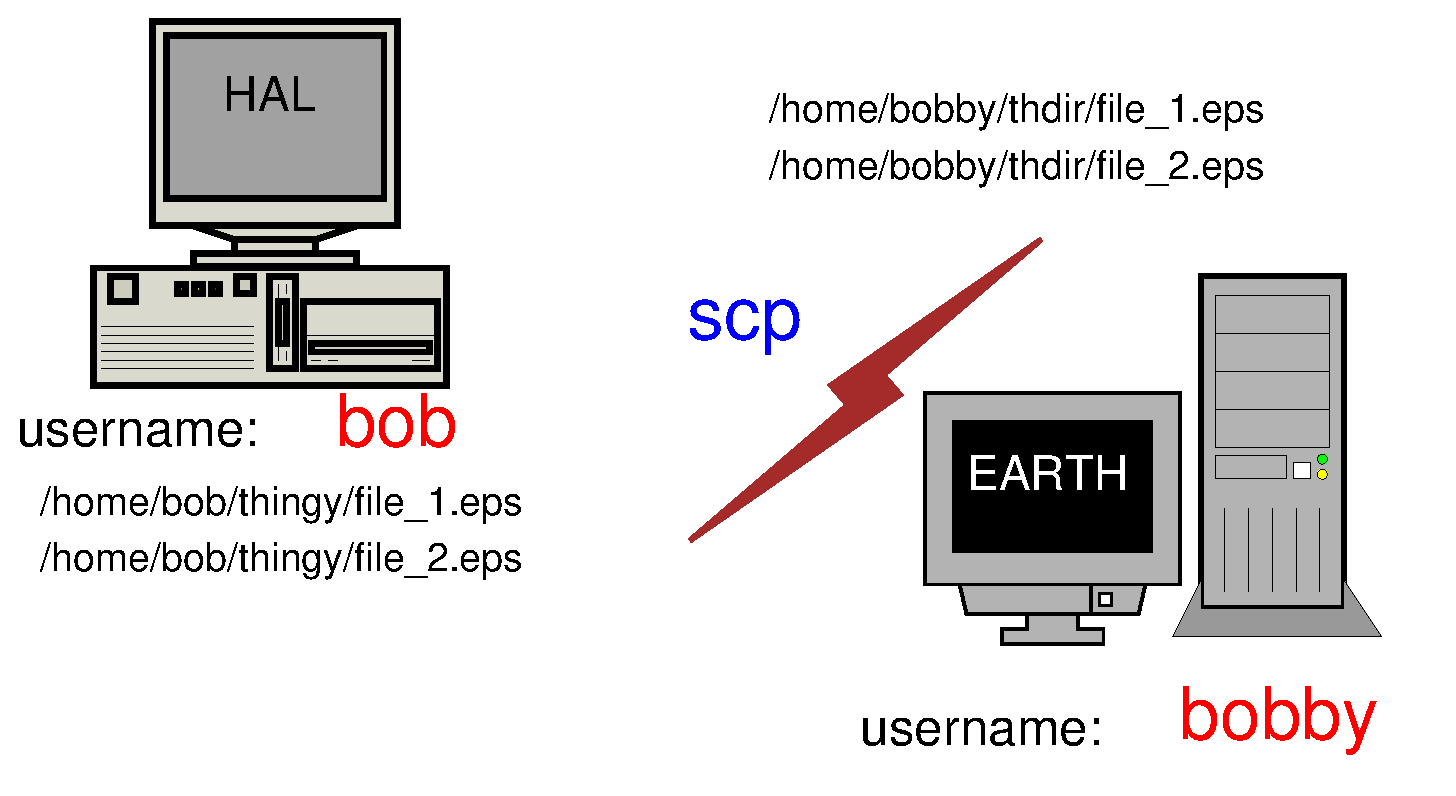
\includegraphics[angle=0,width=5cm]{./Figs/Diagram4.eps}%}
\end{center}
\end{columns}
}
  \end{block}
  
%%%%%%%%%%%%%%%%%%%%%%%%%%%%%%%%%%%%%%%%%%%%%%%%%%%%%%%%%%%%%%%%%%%%%%%%%%%%%%%%%%
\note{
{\tiny

Notes Module V
}
}
\end{frame}
%%%%%%%%%%%%%%%%%%%%%%%%%%%%%%%%%%%%%%%%%%%%%%%%%%%%%%%%%%%%%%%%%%%%%%%%%%%% 
%%%%%%%%%%%%%%%%%%%%%%%%%%%%%%%%%%%%%%%%%%%%%%%%%%%%%%%%%%%%%%%%%%%%%%%%%%%% 
\begin{frame}[t,fragile]{Using \alert{\texttt{scp}} for secure file transfer}
  % ------------------------------------------------------


  \begin{block}{Command syntax: \alert{\texttt{scp} \emph{user1}@\emph{host1:file1}  \emph{user2}@\emph{host2:[file2|dir2]}}}
    {\footnotesize  To transfer from \texttt{hal} to \texttt{earth} the files in the example the syntax is}
{\scriptsize
  \begin{lstlisting}
bob@hal:~$ scp thingy/file_1.eps     bobby@earth:thdir
Password: 
file_1.eps  100%  581     0.6KB/s   00:00    
bob@hal:~$ scp thingy/file_2.eps     bobby@earth:thdir
Password: 
file_2.eps  100%  581     0.6KB/s   00:00    
  \end{lstlisting}
}

{\footnotesize\textbf{(a)}  We have assumed that the remote directory \texttt{thdir} exists. In case it does not exist use the \alert{\texttt{-r}} option. This option also allows the recursive copy of folders and its contents.\\
\textbf{(b)} Wildcards and globbing works in the same way as with the usual \texttt{cp} command.
}

  \end{block}
  
%%%%%%%%%%%%%%%%%%%%%%%%%%%%%%%%%%%%%%%%%%%%%%%%%%%%%%%%%%%%%%%%%%%%%%%%%%%%%%%%%%
\note{
{\tiny

Notes Module V
}
}
\end{frame}
%%%%%%%%%%%%%%%%%%%%%%%%%%%%%%%%%%%%%%%%%%%%%%%%%%%%%%%%%%%%%%%%%%%%%%%%%%%% 
%%%%%%%%%%%%%%%%%%%%%%%%%%%%%%%%%%%%%%%%%%%%%%%%%%%%%%%%%%%%%%%%%%%%%%%%%%%% 
%%%%%%%%%%%%%%%%%%%%%%%%%%%%%%%%%%%%%%%%%%%%%%%%%%%%%%%%%%%%%%%%%%%%%%%%%%%% 
%%%%%%%%%%%%%%%%%%%%%%%%%%%%%%%%%%%%%%%%%%%%%%%%%%%%%%%%%%%%%%%%%%%%%%%%%%%% 
%%%%%%%%%%%%%%%%%%%%%%%%%%%%%%%%%%%%%%%%%%%%%%%%%%%%%%%%%%%%%%%%%%%%%%%%%%%% 
%%%%%%%%%%%%%%%%%%%%%%%%%%%%%%%%%%%%%%%%%%%%%%%%%%%%%%%%%%%%%%%%%%%%%%%%%%%% 
\section{A (Very Basic) Primer on git}
%%%%%%%%%%%%%%%%%%%%%%%%%%%%%%%%%%%%%%%%%%%%%%%%%%%%%%%%%%%%%%%%%%%%%%%%%%%% 
%%%%%%%%%%%%%%%%%%%%%%%%%%%%%%%%%%%%%%%%%%%%%%%%%%%%%%%%%%%%%%%%%%%%%%%%%%%% 
%%%%%%%%%%%%%%%%%%%%%%%%%%%%%%%%%%%%%%%%%%%%%%%%%%%%%%%%%%%%%%%%%%%%%%%%%%%% 
%%%%%%%%%%%%%%%%%%%%%%%%%%%%%%%%%%%%%%%%%%%%%%%%%%%%%%%%%%%%%%%%%%%%%%%%%%%% 
\begin{frame}[t,fragile]{What the heck is a \alert{Version Control System}?}
  % ------------------------------------------------------
  \begin{block}{Version Control System}
    {\footnotesize
      Provides an automatic way to \textbf{track changes} in software (or any other) projects and \textbf{collaborate} easily and conveniently with others. Gives the power to \textbf{recover or view previous versions} of files and directories without tampering with the main development. Helps to securely \textbf{backup} the project and its history.

      Examples: \texttt{RCS}, \texttt{CVS}, and \texttt{Subversion}; current alternatives, including \texttt{Perforce}, \texttt{Bazaar}, \texttt{Mercurial}, and... \texttt{Git}.}
  \end{block}

  \begin{block}{The GIT Version Control System}
    {\footnotesize
    Developed by GNU/Linux creator \emph{Linus Torvalds} to host the Linux kernel. \texttt{Git} is a \textbf{\emph{command-line} distributed VCS} that is designed in the Unix tradition with a combination of power, speed, and community adoption. The set of commands needed to be productive is relatively small; though mastering \texttt{Git} can be quite complex. We focus on the essential commands.
 }
  \end{block}
  
%%%%%%%%%%%%%%%%%%%%%%%%%%%%%%%%%%%%%%%%%%%%%%%%%%%%%%%%%%%%%%%%%%%%%%%%%%%%%%%%%%
\note{
{\tiny


Notes Module V
}
}
\end{frame}
%%%%%%%%%%%%%%%%%%%%%%%%%%%%%%%%%%%%%%%%%%%%%%%%%%%%%%%%%%%%%%%%%%%%%%%%%%%% 
%%%%%%%%%%%%%%%%%%%%%%%%%%%%%%%%%%%%%%%%%%%%%%%%%%%%%%%%%%%%%%%%%%%%%%%%%%%%
%%%%%%%%%%%%%%%%%%%%%%%%%%%%%%%%%%%%%%%%%%%%%%%%%%%%%%%%%%%%%%%%%%%%%%%%%%%% 
%%%%%%%%%%%%%%%%%%%%%%%%%%%%%%%%%%%%%%%%%%%%%%%%%%%%%%%%%%%%%%%%%%%%%%%%%%%%
\begin{frame}[t,fragile]{The Git Ecosystem}
  \vspace{-0.7cm}
  % ------------------------------------------------------
  \begin{columns}
      \column{.25\textwidth}
      \begin{center}
        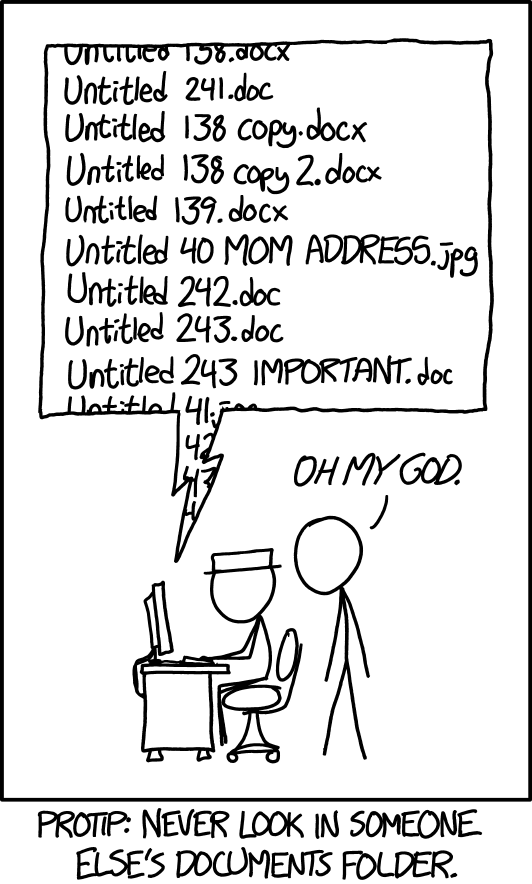
\includegraphics[angle=0,width=\linewidth]{./Figs/git_0.png}
      \end{center}
      \column{.75\textwidth}
      \begin{center}
        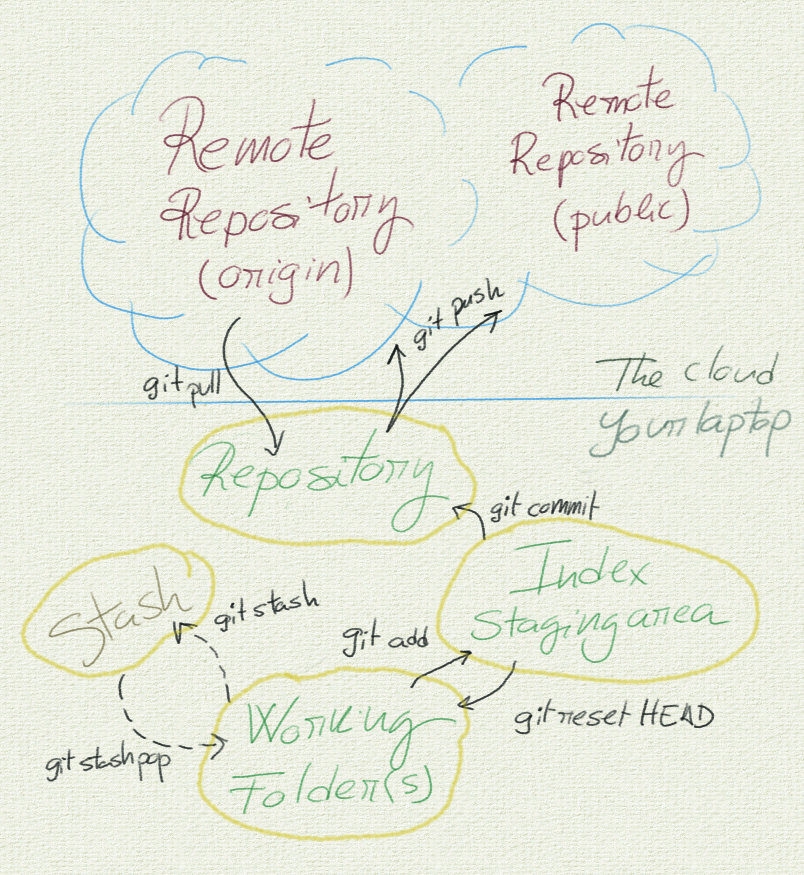
\includegraphics[angle=0,width=0.8\linewidth]{./Figs/git_scheme.png}
      \end{center}
    \end{columns}
  
  %%%%%%%%%%%%%%%%%%%%%%%%%%%%%%%%%%%%%%%%%%%%%%%%%%%%%%%%%%%%%%%%%%%%%%%%%%%%%%%%%% 
  \note{
    {\tiny
      
      Notes Module V
    }
  }
\end{frame}
%%%%%%%%%%%%%%%%%%%%%%%%%%%%%%%%%%%%%%%%%%%%%%%%%%%%%%%%%%%%%%%%%%%%%%%%%%%% 
%%%%%%%%%%%%%%%%%%%%%%%%%%%%%%%%%%%%%%%%%%%%%%%%%%%%%%%%%%%%%%%%%%%%%%%%%%%%
%%%%%%%%%%%%%%%%%%%%%%%%%%%%%%%%%%%%%%%%%%%%%%%%%%%%%%%%%%%%%%%%%%%%%%%%%%%% 
%%%%%%%%%%%%%%%%%%%%%%%%%%%%%%%%%%%%%%%%%%%%%%%%%%%%%%%%%%%%%%%%%%%%%%%%%%%% 
%%%%%%%%%%%%%%%%%%%%%%%%%%%%%%%%%%%%%%%%%%%%%%%%%%%%%%%%%%%%%%%%%%%%%%%%%%%%
\begin{frame}[t,fragile]{Git Configuration and Starting a Git project}
  % ------------------------------------------------------
%  {\small
    \alert{Global configuration} (only once).
    \begin{lstlisting}
      $ git config --global user.name "Bob Mc User"
      $ git config --global user.emil "bob@uhu.es"
    \end{lstlisting}%}

  \begin{columns}
    \column{.75\textwidth}
    {\scriptsize
      \begin{itemize}
      \item \alert{Starting} a project in a \alert{local} repository
      \begin{lstlisting}
        $ git init [project name]
      \end{lstlisting}

      If the argument is given, creates a folder with this name and the project inside. Otherwise creates the project in the current folder.
      
      \item \alert{Starting} a project from a \alert{remote} repository
      \begin{lstlisting}
        $ git clone [project URL]
      \end{lstlisting}
    \item \alert{Ignoring} files: \texttt{.gitignore}
      \begin{lstlisting}
        $ cat .gitignore
        *.aux
        *.log
        *~
       \end{lstlisting}
       % $      
      \end{itemize}
    }
    \column{.25\textwidth}
    \begin{center}
      
\includegraphics[angle=0,width=\textwidth]{./Figs/git.png}%}
    \end{center}
  \end{columns}
  
  
  %%%%%%%%%%%%%%%%%%%%%%%%%%%%%%%%%%%%%%%%%%%%%%%%%%%%%%%%%%%%%%%%%%%%%%%%%%%%%%%%%% 
  \note{
    {\tiny
      
      Notes Module V
    }
  }
\end{frame}
%%%%%%%%%%%%%%%%%%%%%%%%%%%%%%%%%%%%%%%%%%%%%%%%%%%%%%%%%%%%%%%%%%%%%%%%%%% 
%%%%%%%%%%%%%%%%%%%%%%%%%%%%%%%%%%%%%%%%%%%%%%%%%%%%%%%%%%%%%%%%%%%%%%%%%%%% 
\begin{frame}[t,fragile]{Git Most Common Commands: \alert{\texttt{git status}}}
  % ------------------------------------------------------
      \begin{block}{\alert{\texttt{git status}}: Display project status}
          {\scriptsize 
          \begin{lstlisting}
$ git status
On branch master
Your branch is up to date with 'origin/master'.

Changes not staged for commit:
(use "git add <file>..." to update what will be committed)
(use "git checkout -- <file>..." to discard changes in working directory)

	modified:   gnu_linux_V.tex

Untracked files:
  (use "git add <file>..." to include in what will be committed)

	Figs/Diagram1-eps-converted-to.pdf
	Figs/Diagram1.dia

\end{lstlisting}
%$
}      
\end{block}  
  
  %%%%%%%%%%%%%%%%%%%%%%%%%%%%%%%%%%%%%%%%%%%%%%%%%%%%%%%%%%%%%%%%%%%%%%%%%%%%%%%%%% 
  \note{
    {\tiny
      
      Notes Module V
    }
  }
\end{frame}
%%%%%%%%%%%%%%%%%%%%%%%%%%%%%%%%%%%%%%%%%%%%%%%%%%%%%%%%%%%%%%%%%%%%%%%%%%%% 
%%%%%%%%%%%%%%%%%%%%%%%%%%%%%%%%%%%%%%%%%%%%%%%%%%%%%%%%%%%%%%%%%%%%%%%%%%% 
%%%%%%%%%%%%%%%%%%%%%%%%%%%%%%%%%%%%%%%%%%%%%%%%%%%%%%%%%%%%%%%%%%%%%%%%%%%% 
\begin{frame}[t,fragile]{Git Most Common Commands : \alert{\texttt{git add/reset}}}
  % ------------------------------------------------------
      \begin{block}{\alert{\texttt{git add} \emph{file(s)}}: Send file(s) to the \alert{staging} area}
          {\scriptsize 
          \begin{lstlisting}
$ git add gnu_linux_V.tex 
$ git status
On branch master
Your branch is up to date with 'origin/master'.
Changes to be committed:
  (use "git reset HEAD <file>..." to unstage)
	modified:   gnu_linux_V.tex
Untracked files:
  (use "git add <file>..." to include in what will be committed)
	Figs/Diagram1-eps-converted-to.pdf
	Figs/Diagram1.dia
\end{lstlisting}
%
}
\alert{\texttt{git reset} \emph{[file(s)]}}: removes files from staging area and send them back to working area.

\end{block}  
  
  %%%%%%%%%%%%%%%%%%%%%%%%%%%%%%%%%%%%%%%%%%%%%%%%%%%%%%%%%%%%%%%%%%%%%%%%%%%%%%%%%% 
  \note{
    {\tiny
      
      Notes Module V
    }
  }
\end{frame}
%%%%%%%%%%%%%%%%%%%%%%%%%%%%%%%%%%%%%%%%%%%%%%%%%%%%%%%%%%%%%%%%%%%%%%%%%%%% 
%%%%%%%%%%%%%%%%%%%%%%%%%%%%%%%%%%%%%%%%%%%%%%%%%%%%%%%%%%%%%%%%%%%%%%%%%%% 
%%%%%%%%%%%%%%%%%%%%%%%%%%%%%%%%%%%%%%%%%%%%%%%%%%%%%%%%%%%%%%%%%%%%%%%%%%%% 
\begin{frame}[t,fragile]{Git Most Common Commands : \alert{\texttt{git commit}}}
  % ------------------------------------------------------
  \begin{block}{\alert{\texttt{git commit}}: Create a new commit in the repository. }
      \begin{itemize}
      \item  {\footnotesize The commit includes all changes saved in the \alert{staging area}.
      \begin{lstlisting}
$ git commit 
[master c1fbce5] Test commit. 	modified:   gnu_linux_V.tex
1 file changed, 37 insertions(+)
      \end{lstlisting}
      % $
    }
      \end{itemize}

  \begin{columns}
    \column{.5\textwidth}
      \begin{itemize}
  \item  {\scriptsize Every commit \alert{must} have a message.
      }
  \item  {\scriptsize Commit often and verbosely.
      }
  \item  {\scriptsize Every commit has a unique identifier.
      }
  \item  {\scriptsize Option \texttt{-m}: inline statement message. 
      }
      \end{itemize}
    \column{.5\textwidth}
    \begin{center}
      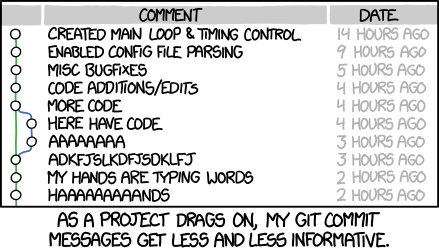
\includegraphics[angle=0,width=0.9\textwidth]{./Figs/git_commit.png}%}
    \end{center}
  \end{columns}
  
}      
\end{block}  
  
  %%%%%%%%%%%%%%%%%%%%%%%%%%%%%%%%%%%%%%%%%%%%%%%%%%%%%%%%%%%%%%%%%%%%%%%%%%%%%%%%%% 
  \note{
    {\tiny
      
      Notes Module V
    }
  }
\end{frame}
%%%%%%%%%%%%%%%%%%%%%%%%%%%%%%%%%%%%%%%%%%%%%%%%%%%%%%%%%%%%%%%%%%%%%%%%%%%%  
%%%%%%%%%%%%%%%%%%%%%%%%%%%%%%%%%%%%%%%%%%%%%%%%%%%%%%%%%%%%%%%%%%%%%%%%%%% 
%%%%%%%%%%%%%%%%%%%%%%%%%%%%%%%%%%%%%%%%%%%%%%%%%%%%%%%%%%%%%%%%%%%%%%%%%%%% 
\begin{frame}[t,fragile]{Git Most Common Commands : \alert{\texttt{git diff}}}
  % ------------------------------------------------------
      \begin{block}{\alert{\texttt{git diff [--staged]} \emph{[file(s)]}}: Show changes}
        {\scriptsize
          By default it shows changes between \alert{working} and \alert{staging} areas. If no change is staged, show differences wrt \alert{repository} area.
          \begin{lstlisting}
$ git diff
diff --git a/gnu_linux_V.tex b/gnu_linux_V.tex
index 1c85e18..49af047 100644
--- a/gnu_linux_V.tex
+++ b/gnu_linux_V.tex
@@ -608,12 +608,11 @@ Notes Module V
...
\end{lstlisting}
%$
The option \alert{\texttt{--staged}} show differences between staged and repository contents.

Differences between the index and a tree, between two trees, between two blob objects, or between two files on disk can also be shown.}      
\end{block}  
  
  %%%%%%%%%%%%%%%%%%%%%%%%%%%%%%%%%%%%%%%%%%%%%%%%%%%%%%%%%%%%%%%%%%%%%%%%%%%%%%%%%% 
  \note{
    {\tiny
      
      Notes Module V
    }
  }
\end{frame}
%%%%%%%%%%%%%%%%%%%%%%%%%%%%%%%%%%%%%%%%%%%%%%%%%%%%%%%%%%%%%%%%%%%%%%%%%%%% 
%%%%%%%%%%%%%%%%%%%%%%%%%%%%%%%%%%%%%%%%%%%%%%%%%%%%%%%%%%%%%%%%%%%%%%%%%%%
%%%%%%%%%%%%%%%%%%%%%%%%%%%%%%%%%%%%%%%%%%%%%%%%%%%%%%%%%%%%%%%%%%%%%%%%%%%%  
%%%%%%%%%%%%%%%%%%%%%%%%%%%%%%%%%%%%%%%%%%%%%%%%%%%%%%%%%%%%%%%%%%%%%%%%%%% 
%%%%%%%%%%%%%%%%%%%%%%%%%%%%%%%%%%%%%%%%%%%%%%%%%%%%%%%%%%%%%%%%%%%%%%%%%%%% 
\begin{frame}[t,fragile]{Git Most Common Commands : \alert{\texttt{git log}}}
  % ------------------------------------------------------
      \begin{block}{\alert{\texttt{git log [-n \emph{count}]}}: List history of current branch}
        {\scriptsize
          The option \texttt{-n \emph{count}} limits the list to the last \emph{n} commits. 
          \begin{lstlisting}
$ git log -n 1
commit 73f235c202932583db254eaf8212b7 (HEAD -> master, origin/master)
Author: Curro Perez-Bernal <currix@gmail.com>
Date:   Mon May 18 00:43:30 2020 +0200

    Added some git slides: diff add/reset commit
            modified:   gnu_linux_V.tex
\end{lstlisting}
%$
\begin{itemize}
  \item A convenient way to get an overview of the project is with  the command

\texttt{git log --oneline --graph --decorate}

          \begin{lstlisting}
$ git log --oneline --graph --decorate
* 73f235c (HEAD -> master, origin/master) Added some git slides: \
diff add/reset commit  modified:   gnu_linux_V.tex
* c1fbce5 Test commit.  modified:   gnu_linux_V.tex
* 1994bf9 Typos in user add and silent login added to ssh.
* 26fad37 Changes to update to 2020 course.
\end{lstlisting}
%$
\end{itemize}
}
\end{block}  
  
  %%%%%%%%%%%%%%%%%%%%%%%%%%%%%%%%%%%%%%%%%%%%%%%%%%%%%%%%%%%%%%%%%%%%%%%%%%%%%%%%%% 
  \note{
    {\tiny
      
      Notes Module V
    }
  }
\end{frame}
%%%%%%%%%%%%%%%%%%%%%%%%%%%%%%%%%%%%%%%%%%%%%%%%%%%%%%%%%%%%%%%%%%%%%%%%%%%% 
%%%%%%%%%%%%%%%%%%%%%%%%%%%%%%%%%%%%%%%%%%%%%%%%%%%%%%%%%%%%%%%%%%%%%%%%%%%
%%%%%%%%%%%%%%%%%%%%%%%%%%%%%%%%%%%%%%%%%%%%%%%%%%%%%%%%%%%%%%%%%%%%%%%%%%% 
%%%%%%%%%%%%%%%%%%%%%%%%%%%%%%%%%%%%%%%%%%%%%%%%%%%%%%%%%%%%%%%%%%%%%%%%%%%% 
\begin{frame}[t,fragile]{Git Most Common Commands : \alert{\texttt{git checkout}}}
  % ------------------------------------------------------
      \begin{block}{\alert{\texttt{git checkout {-}{-}} \emph{[file(s)]}}: Discard changes in working area}
        {\scriptsize
          Discard changes in \alert{working} area and recover file or files in \alert{repository} area. 
          \begin{lstlisting}
$ ls -l gnu_linux_IV.tex
-rw-r--r-- 1 curro curro 20219 May 18 12:00 gnu_linux_IV.tex
$ git checkout -- gnu_linux_IV.tex
$ ls -l gnu_linux_IV.tex
-rw-r--r-- 1 curro curro 20531 May 18 12:00 gnu_linux_IV.tex
\end{lstlisting}
%$
\begin{itemize}
  \item Notice that this operation is  \alert{unrecoverable}.

\item The \texttt{--} option is to avoid conflicts between paths and options.

\item You can also chose to check out files from a particular commit:

\texttt{git checkout c1fbce52 {-}{-} gnu\_linux\_IV.tex}.
\end{itemize}
}      
\end{block}  
  
  %%%%%%%%%%%%%%%%%%%%%%%%%%%%%%%%%%%%%%%%%%%%%%%%%%%%%%%%%%%%%%%%%%%%%%%%%%%%%%%%%% 
  \note{
    {\tiny
      
      Notes Module V
    }
  }
\end{frame}
%%%%%%%%%%%%%%%%%%%%%%%%%%%%%%%%%%%%%%%%%%%%%%%%%%%%%%%%%%%%%%%%%%%%%%%%%%%% 
%%%%%%%%%%%%%%%%%%%%%%%%%%%%%%%%%%%%%%%%%%%%%%%%%%%%%%%%%%%%%%%%%%%%%%%%%%%
%%%%%%%%%%%%%%%%%%%%%%%%%%%%%%%%%%%%%%%%%%%%%%%%%%%%%%%%%%%%%%%%%%%%%%%%%%% 
%%%%%%%%%%%%%%%%%%%%%%%%%%%%%%%%%%%%%%%%%%%%%%%%%%%%%%%%%%%%%%%%%%%%%%%%%%%% 
\begin{frame}[t,fragile]{Git Most Common Commands : \alert{\texttt{git push}} and \alert{\texttt{git pull}}}
  % ------------------------------------------------------
      \begin{block}{Commands for \emph{remote repository synchronization}}
        {\scriptsize
\begin{itemize}
  \item          The command  \alert{\texttt{git push [remote]}} pushes local changes to the remote repository.
          \begin{lstlisting}
$ git push
Enumerating objects: 5, done.
Counting objects: 100% (5/5), done.
Delta compression using up to 4 threads
Compressing objects: 100% (3/3), done.
Writing objects: 100% (3/3), 1.35 KiB | 460.00 KiB/s, done.
Total 3 (delta 2), reused 0 (delta 0)
remote: Resolving deltas: 100% (2/2), completed with 2 local objects.
To https://github.com/currix/GNU_Linux_Slides.git
   73f235c..9802fe4  master -> master
\end{lstlisting}
%$
  \item  The command  \alert{\texttt{git pull [remote]}} fetches changes from the remote repository to the local repository, merging the current branch with its upstreams.
          \begin{lstlisting}
$ git pull
Already up to date.
\end{lstlisting}
%$
\end{itemize}
}
\end{block}  
  
  %%%%%%%%%%%%%%%%%%%%%%%%%%%%%%%%%%%%%%%%%%%%%%%%%%%%%%%%%%%%%%%%%%%%%%%%%%%%%%%%%% 
  \note{
    {\tiny
      
      Notes Module V
    }
  }
\end{frame}


%%%%%%%%%
\end{document}
